% Presupposition CogSci 2016

\begin{figure*}
 \centering
  \subfigure[QUD$_\text{max}$]{\label{fig:RSA_QUDmax}
  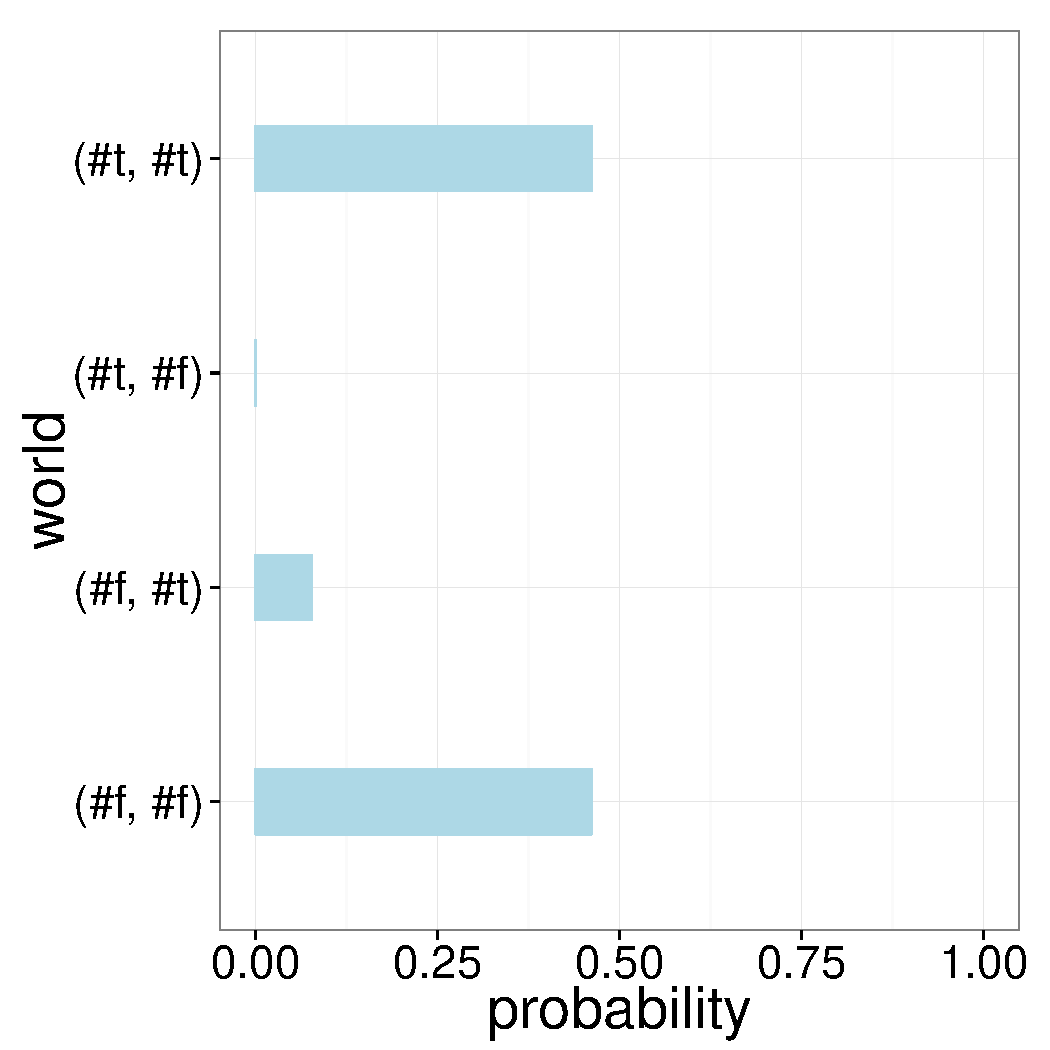
\includegraphics[scale=0.23]{figs/CGprior.pdf}}
  \subfigure[QUD$_\text{now}$]{\label{fig:RSA_QUDnow2}
  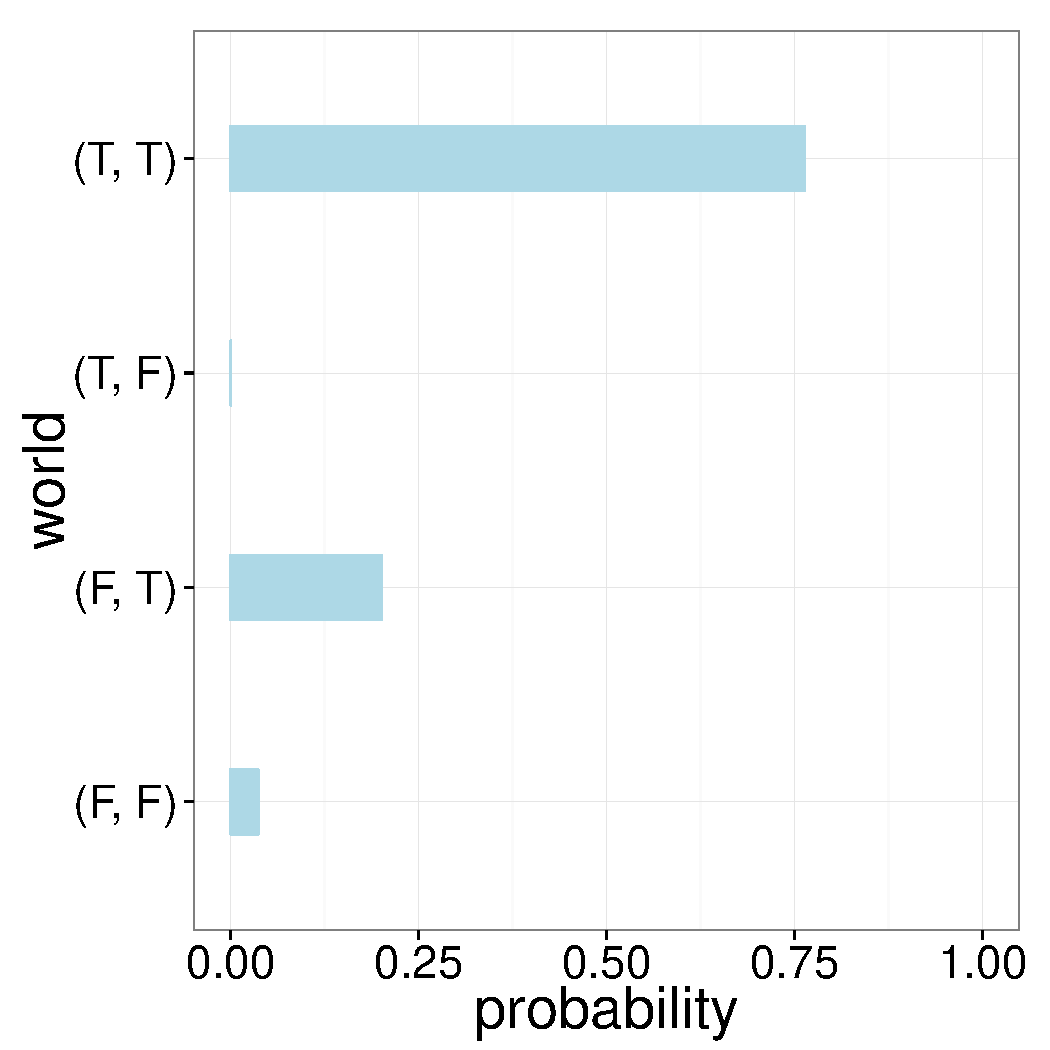
\includegraphics[scale=0.23]{figs/QUDnow.pdf}}
  \subfigure[QUD$_\text{past}$]{\label{fig:RSA_QUDpast}
    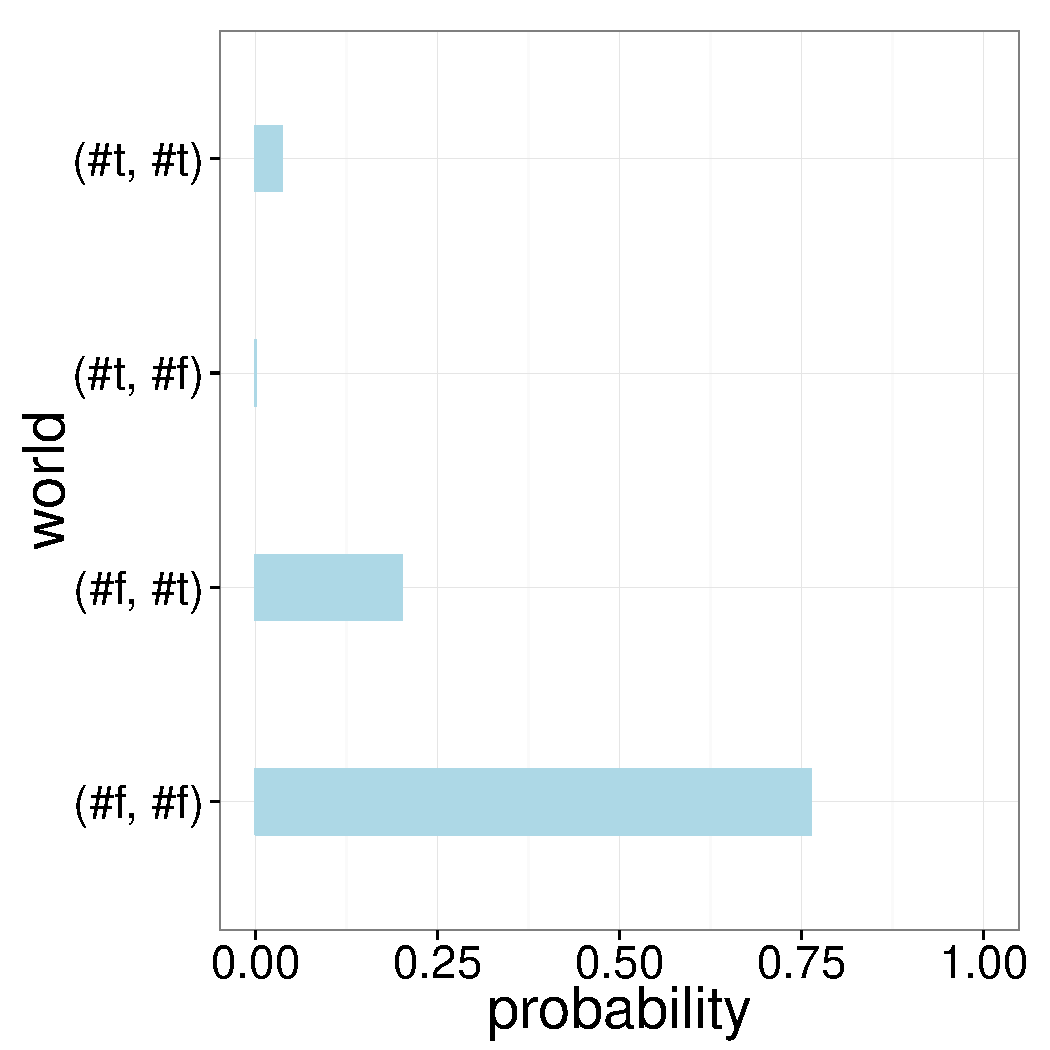
\includegraphics[scale=0.23]{figs/QUDpast.pdf}}
  \subfigure[QUD$_\text{change}$]{\label{fig:RSA_QUDchange}
    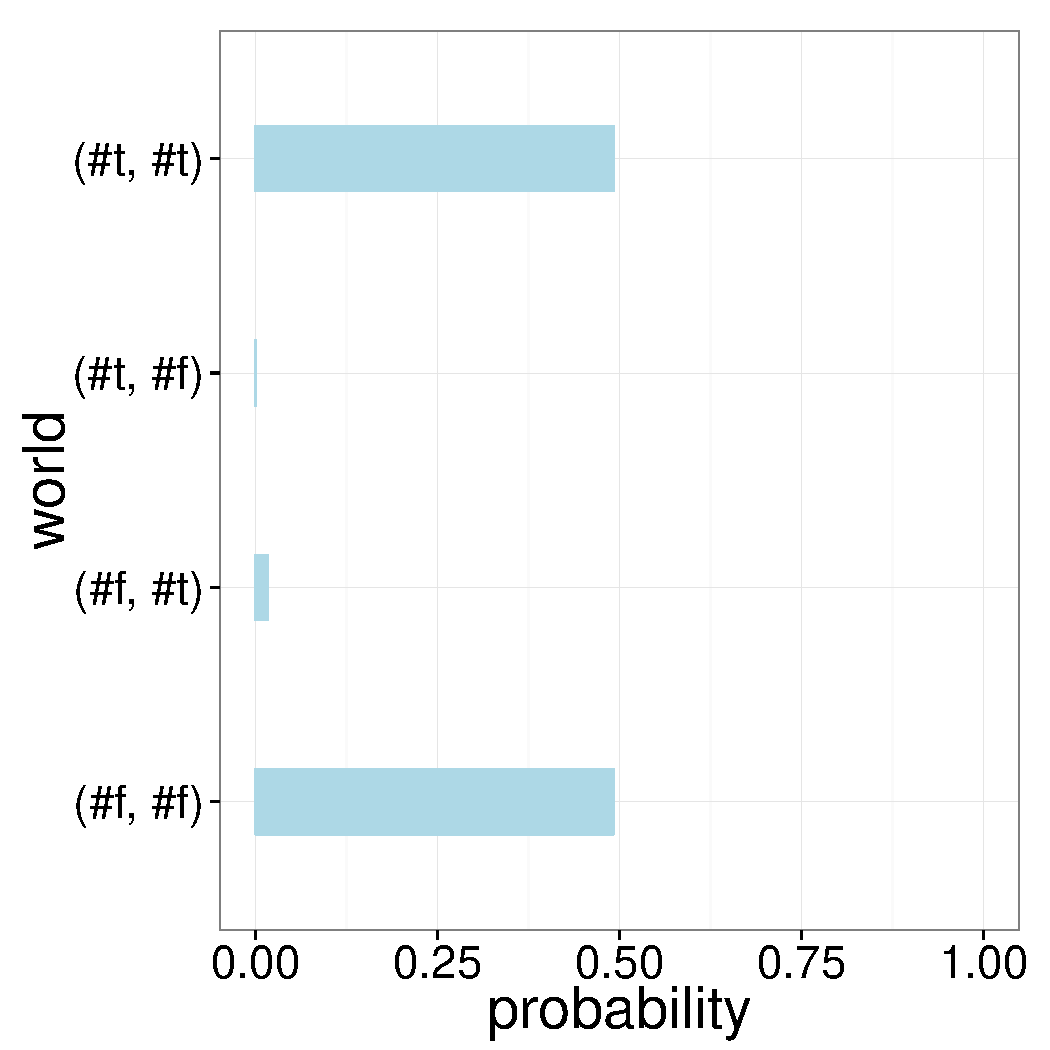
\includegraphics[scale=0.23]{figs/QUDchange.pdf}}
  
 \subfigure[QUD$_\text{always}$]{\label{fig:RSA_QUDalways}
 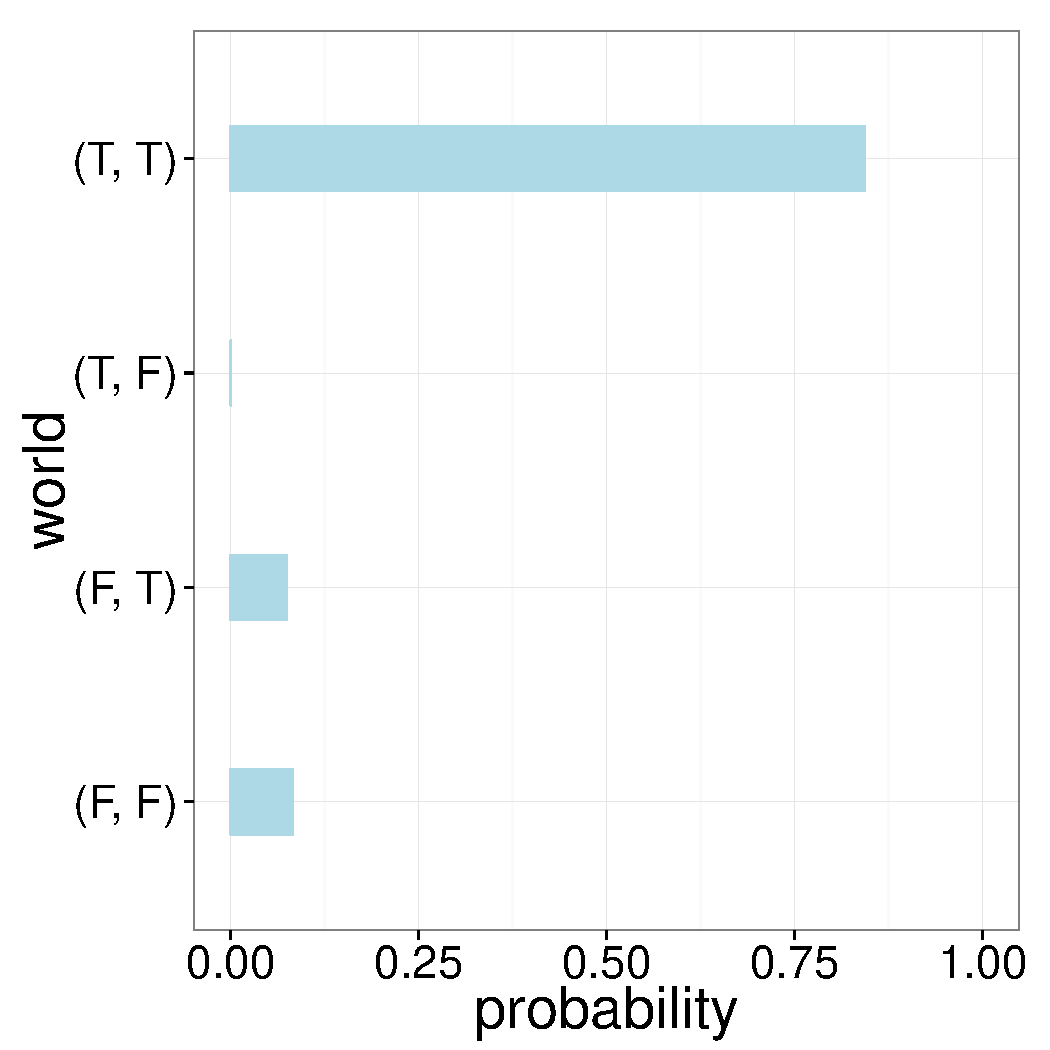
\includegraphics[scale=0.23]{figs/QUDalways.pdf}}
 \subfigure[QUD$_\text{stop}$]{\label{fig:RSA_QUDstop}
 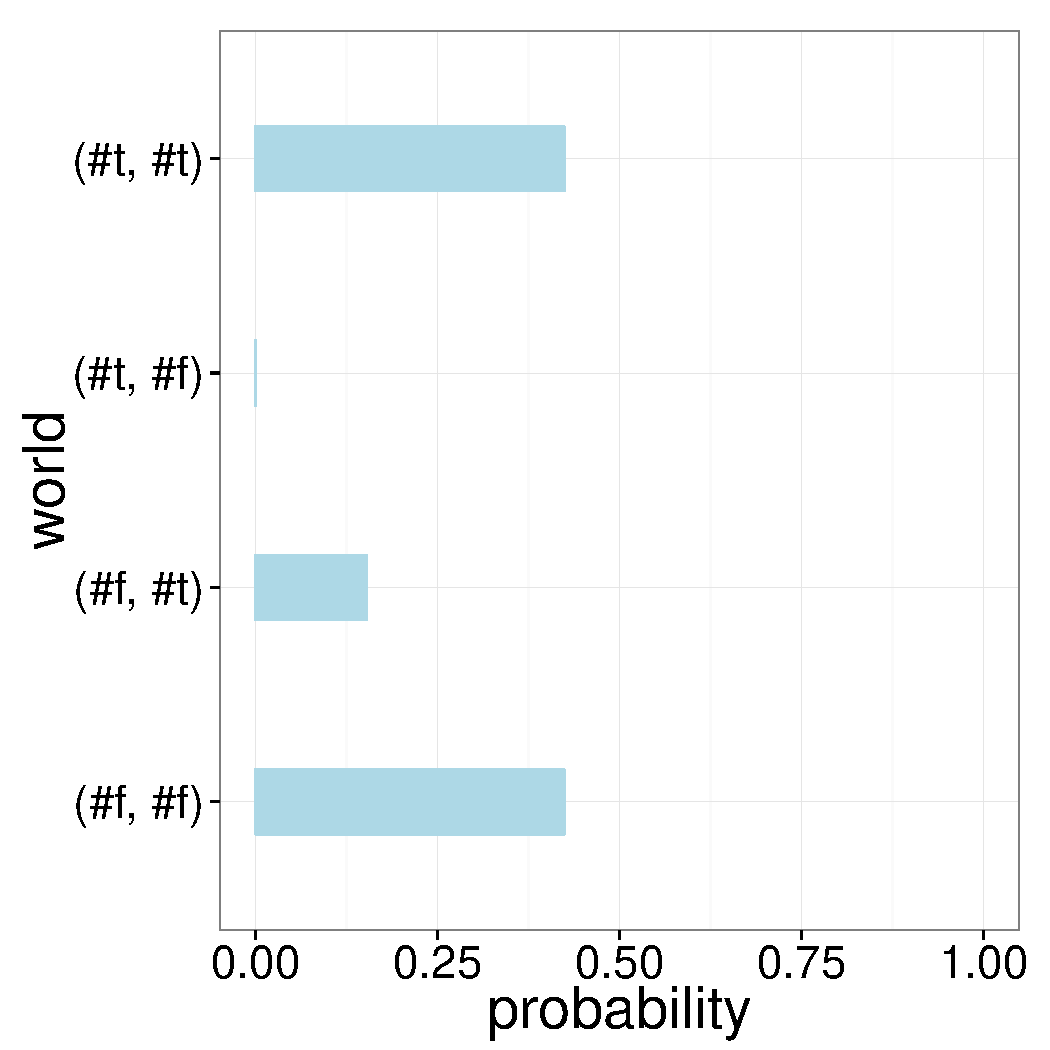
\includegraphics[scale=0.23]{figs/QUDstop.pdf}}
 \subfigure[QUD$_\text{start}$]{\label{fig:RSA_QUDstart}
   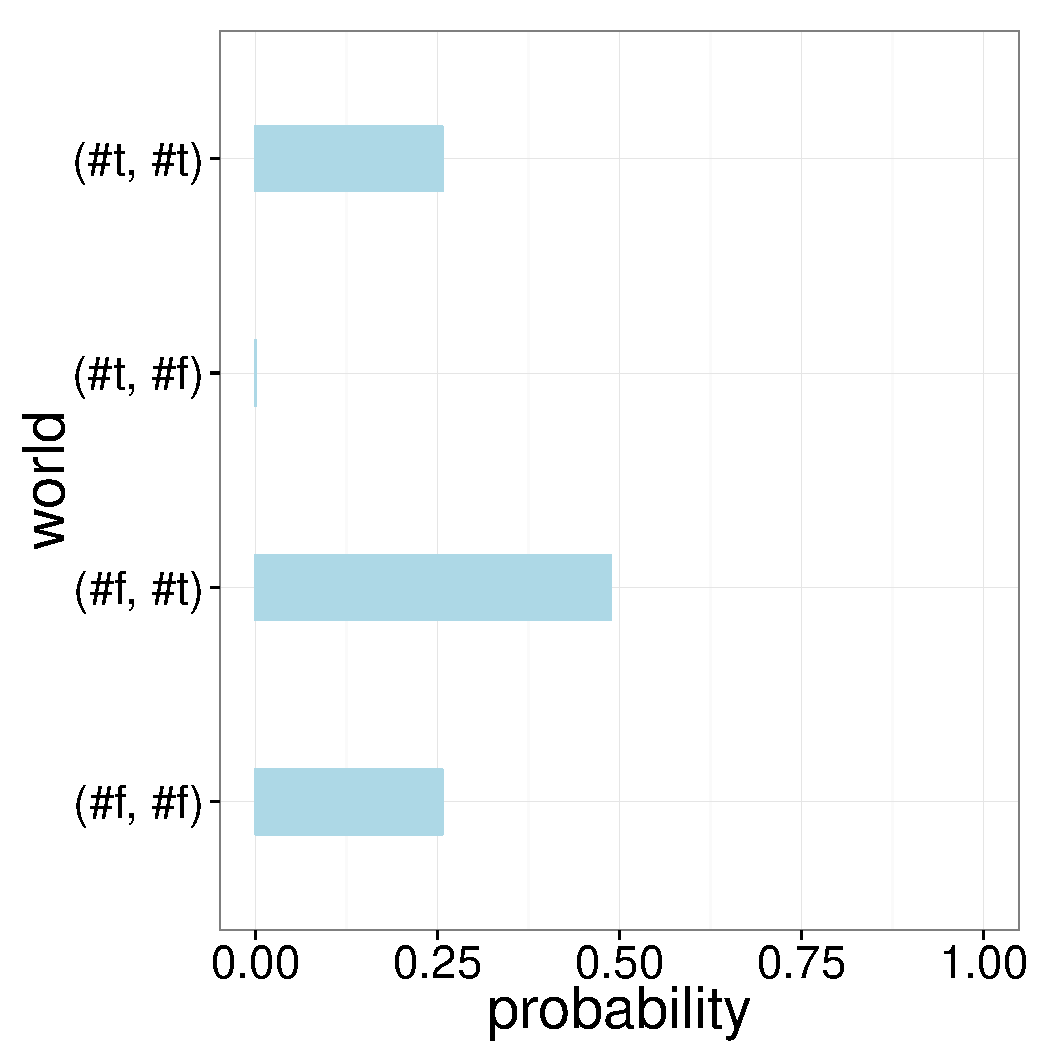
\includegraphics[scale=0.23]{figs/QUDstart.pdf}}
 \subfigure[QUD$_\text{never}$]{\label{fig:RSA_QUDnever}
   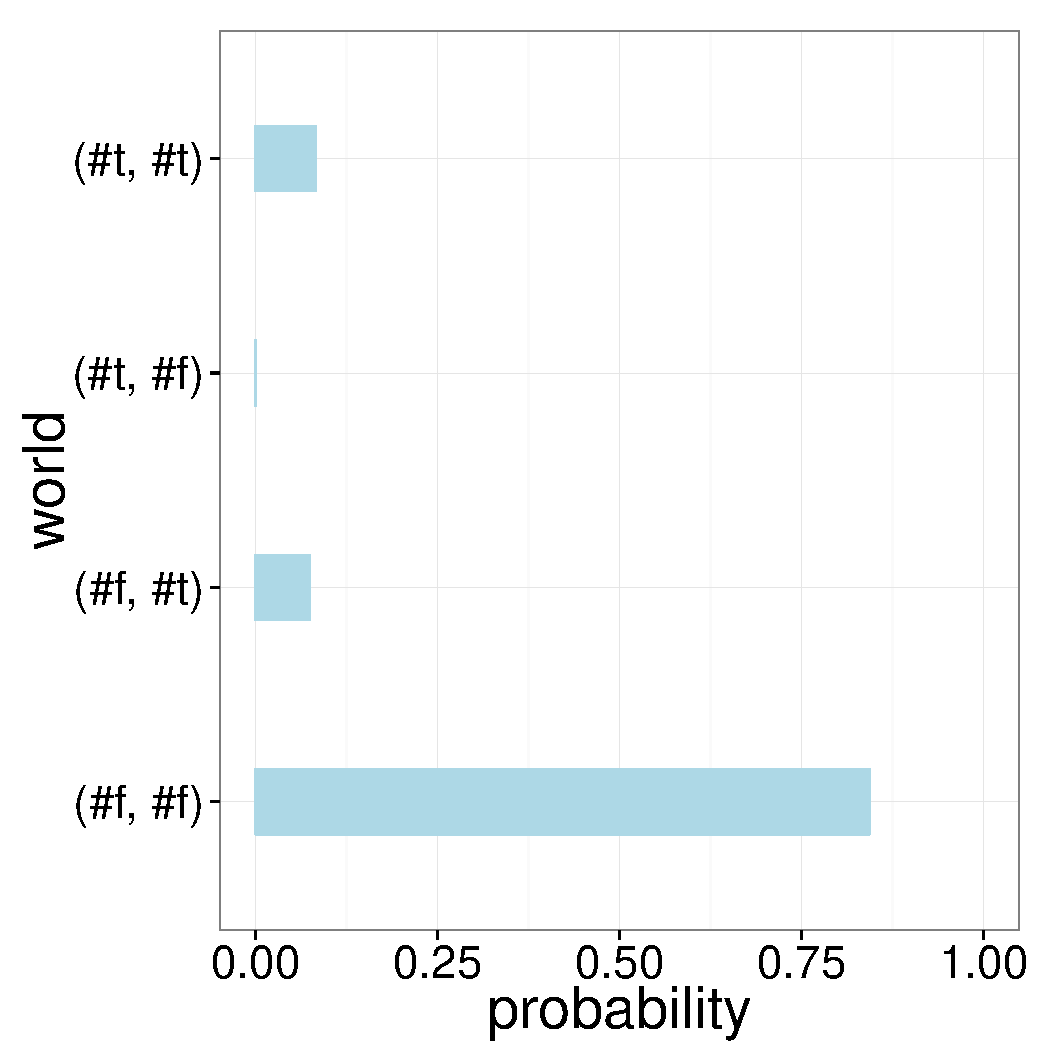
\includegraphics[scale=0.23]{figs/QUDnever.pdf}}
\vspace{-1ex}
 \caption{Pragmatic listener after hearing ``John did not stop smoking'' for different QUDs, with $\alpha=6$ and CG prior \label{fig:RSA_QUDs}}
\vspace{-6ex}
\end{figure*}


We have introduced a RSA model with common ground and shown its
 predictions for QUD$_\textrm{now}$ and QUD$_\textrm{max}$.
The prediction is sensitive to the QUD---in Figure~\ref{fig:RSA_QUDs} we show predictions for eight different QUDs.
%In this section, we further explore the interaction between the QUD and projection
% predicted by the model. 
%Concretely, besides QUD$_\textrm{max}$, we consider all 7 QUDs with yes/no answers: 
% QUD$_\text{now}$, QUD$_\text{past}$, QUD$_\text{change}$,
% QUD$_\text{always}$, QUD$_\text{stop}$, QUD$_\text{start}$, and QUD$_\text{never}$.
%For instance, QUD$_\text{always}$ asks whether it is the case that John both smoked in
% the past and smokes now.
%The predictions of the RSA model for these QUDs are shown in
% Figure~\ref{fig:RSA_QUDs}.
In general, it seems that the model is making plausible predictions. 
For example, when the QUD is whether John has always smoked, ``John did not stop smoking'' implies that John has always smoked (Figure~\ref{fig:RSA_QUDalways}). 
When the QUD is whether John has never smoked, ``John did not stop smoking'' implies that John has never smoked (Figure~\ref{fig:RSA_QUDnever}). 
When the QUD is about whether John stopped smoking (Figure~\ref{fig:RSA_QUDstop}) 
 or there is a change (Figure~\ref{fig:RSA_QUDchange}), after hearing
 ``John did not stop smoking,'' the pragmatic listener still believes that that John 
 smoked in the past is roughly equally likely as that John did not smoke in the past. 
 (Compare this to Geurts' example, described earlier.)
Further experimental data will be needed to assess whether these predictions are borne out.

